\chapter{Lattice based cryptography}\label{Lattice-based-cryptograph}

Lattice based public key encryption (and its cousins known as knapsack
and coding based encryption) have almost as long a history as discrete
logarithm and factoring based schemes. Already in 1976, right after the
Diffie-Hellman key exchange was discovered (and before RSA), Ralph
Merkle was working on building public key encryption from the NP hard
\emph{knapsack} problem (see
\href{http://cr.yp.to/bib/1988/diffie.pdf}{Diffie's recollection}). This
can be thought of as the task of solving a linear equation of the form
\(Ax = y\) (where \(A\) is a given matrix, \(y\) is a given vector, and
the unknown are \(x\)) over the real numbers but with the additional
constraint that \(x\) must be either \(0\) or \(1\). His proposal
evolved into the Merkle-Hellman system proposed in 1978 (which was
broken in 1984).

McEliece proposed in 1978 a system based on the difficulty of the
decoding problem for general linear codes. This is the task of solving
\emph{noisy linear equations} where one is given \(A\) and \(y\) such
that \(y=Ax+e\) for a ``small'' error vector \(e\), and needs to recover
\(x\). Crucially, here we work in a finite field, such as working modulo
\(q\) for some prime \(q\) (that can even be \(2\)) rather than over the
reals or rationals. There are special matrices \(A^*\) for which we know
how to solve this problem efficiently: these are known as efficiently
decodable \href{https://goo.gl/vM7Pvv}{error correcting codes}. McEliece
suggested a scheme where the key generator lets \(A\) be a ``scrambled''
version of a special \(A^*\) (based on the
\href{https://goo.gl/Vd4yye}{Goppa algebraic geometric code}). So,
someone that knows the scrambling could solve the problem, but
(hopefully) someone that doesn't know it wouldn't. McEliece's system has
so far not been broken.

In a 1996 breakthrough, Ajtai showed a \emph{private key} scheme based
on integer lattices that had a very curious property- its security could
be based on the assumption that certain problems were only hard in the
\emph{worst case}, and moreover variants of these problems were known to
be NP hard. This re-ignited the hope that we could perhaps realize the
old dream of basing crypto on the mere assumption that
\(P\neq \ensuremath{\mathit{NP}}\). Alas, we now understand that there
are fundamental barriers to this approach.

Nevertheless, Ajtai's work attracted significant interest, and within a
year both Ajtai and Dwork, as well as Goldreich, Goldwasser and Halevi
came up with lattice based constructions for \emph{public key}
encryption (the former based also on \emph{worst case} assumptions). At
about the same time, Hoffstein, Pipher, and Silverman came up with their
NTRU public key system which is based on stronger assumptions but offers
better performance, and they started a company around it together with
Daniel Lieman.

You may note that I haven't yet said what \emph{lattices} are; we will
do so later, but for now if you simply think of questions involving
linear equations modulo some prime \(q\), you will get enough of the
intuition that you need. (The lattice viewpoint is more geometric, and
we'll discuss it more below; it was first used to \emph{attack}
cryptosystems and in particular break the Merkle-Hellman knapsack scheme
and many of its variants.)

Lattice based cryptography has captured a lot of attention recently from
both theory and practice. In the theory side, many cool new
constructions are now based on lattice based cryptography, and chief
among them fully homomorphic encryption, as well as indistinguishability
obfuscation (though the latter's security's foundations are still far
less solid). On the applied side, the steady advances in the technology
of quantum computers have finally gotten practitioners worried about
RSA, Diffie Hellman and Elliptic Curves. While current constructions for
quantum computers are nowhere near being able to, say, factor larger
numbers that can be done classically (or even than can be done by hand),
given that it takes many years to develop new standards and get them
deployed, many believe the effort to transition away from these
factoring/dlog based schemes should start today (or perhaps should have
started several years ago). The NSA has
\href{https://www.nsa.gov/ia/programs/suiteb_cryptography/index.shtml}{suggested}
that it plans to initiate the process to ``transition to quantum
resistant algorithms in the not too distant future''; see also this
\href{https://cryptome.org/2016/01/CNSA-Suite-and-Quantum-Computing-FAQ.pdf}{very
interesting FAQ} on this topic.

Cryptography has the peculiar/unfortunate feature that if a machine is
built that can factor large integers in 20 years, it can still be used
to break the communication we transmit \emph{today}, provided this
communication was recorded. So, if you have some data that you expect
you'd want still kept secret in 20 years (as many government and
commercial entities do), you might have reasons to worry. Currently
lattice based cryptography is the only real ``game in town'' for
potentially quantum-resistant public key encryption schemes.

Lattice based cryptography is a huge area, and in this lecture and this
course we only touch on few aspects of it. I highly recommend
\href{https://web.eecs.umich.edu/~cpeikert/pubs/lattice-survey.pdf}{Chris
Peikert's Survey} for a much more in depth treatment of this area.

\subsection{Quick linear algebra recap}\label{Quick-linear-algebra-reca}

A \emph{field} \(\mathbb{F}\) is a set that supports the operations
\(+,\cdot\) and contains the numbers \(0\) and \(1\) (more formally the
additive identity and multiplicative identity) with the usual properties
that the real numbers have. (That is associative, commutative, and
distributive law, the fact that for every \(x \in \mathbb{F}\) there is
an element \(-x\) such that \(x + (-x) = 0\) and that if \(x \neq 0\)
there is an element \(x^{-1}\) such that \(x \cdot x^{-1} = 1\).) Apart
from the real numbers, the main field we will be interested in this
section is the field \(\Z_q\) of the numbers \(\{0,1,\ldots,q-1\}\) with
addition and multiplication done modulo \(q\), where \(q\) is a prime
number.\footnote{While this won't be of interest for us in this chapter,
  one can also define finite fields whose size is a \emph{prime power}
  of the form \(q^k\) where \(q\) is a prime and \(k\) is an integer;
  this is sometimes useful and in particular fields of size \(2^k\) are
  sometimes used in practice. In such fields we usually think of the
  elements as \emph{vector} \(v \in (\Z_q)^k\) with addition done
  component-wise but multiplication is not defined component-wise (since
  otherwise a vector with a single coordinate zero would not have an
  inverse) but in a different way, via interpreting these vectors as
  coefficients of a degree \(k-1\) polynomial.}

You should be comfortable with the following notions:

\begin{itemize}
\item
  A vector \(v \in \mathbb{F}^n\) and a \emph{matrix}
  \(M \in \mathbb{F}^{m \times n}\). An \(m\times n\) matrix has \(m\)
  rows and \(n\) columns. We think of vectors as \emph{column vectors}
  and so we can think of a vector \(v \in \mathbb{F}^n\) as an
  \(n\times 1\) matrix. We write the \(i\)-the coordinate of \(v\) as
  \(v_i\) and the \((i,j)\)-th coordinate of \(M\) as \(M_{i,j}\)
  (i.e.~the coordinate in the \(i\)-th row and the \(j\)-th column.) We
  often write a vector \(v\) as \((v_1,\ldots,v_n)\) but we still mean
  that it's a column vector unless we say otherwise.
\item
  If \(\alpha \in \mathbb{F}\) is a \emph{scalar} (i.e., a number) and
  \(v \in \mathbb{F}^n\) is a vector then \(\alpha v\) is the vector
  \((\alpha v_1 ,\ldots, \alpha v_n)\). If \(u,v\) are \(n\) dimensional
  vectors then \(u+v\) is the vector \((u_1+v_1,\ldots,u_n+v_n)\).
\item
  A \emph{linear subspace} \(V \subseteq \mathbb{F}^n\) is a non-empty
  set of vectors such that for every vectors \(u,v \in V\) and
  \(\alpha,\beta \in \mathbb{F}\), \(\alpha u + \beta v \in V\). In
  particular this means that \(V\) contains the all zero vector \(0^n\)
  (can you see why?). A subset \(A \subseteq V\) is \emph{linearly
  independent} if there is no collection \(a_1,\ldots,a_k \in A\) and
  scalars \(\alpha_1,\ldots,\alpha_k\) such that
  \(\sum \alpha_i a_i = 0^n\). It is known (and not hard to prove) that
  if \(A\) is linearly independent then \(|A| \leq n\). It is known that
  for every such linear subspace there is a linearly independent set
  \(B = \{ b_1,\ldots,b_d \}\) of vectors, with \(d \leq n\), such that
  for every \(u \in V\) there exist \(\alpha_1,\ldots,\alpha_d\) such
  that \(v = \sum \alpha_i b_i\). Such a set is known as a \emph{basis}
  for \(V\). A subspace \(V\) has many bases, but all of them have the
  same size \(d\) which is known as the \emph{dimension} of \(V\). An
  \emph{affine subspace} is a set \(U\) of the form
  \(\{ u_0 + v : v\in V \}\) where \(V\) is a linear subspace. We can
  also write \(U\) as \(u_0 + V\). We denote the dimension of \(U\) as
  the dimension of \(V\) in such a case.
\item
  The inner product (also known as ``dot product'')
  \(\langle u,v \rangle\) between two vectors of the same dimension
  \(n\) that is defined as \(\sum u_i v_i\) (addition done in the field
  \(\mathbb{F}\)).\footnote{There is a much more general notion of inner
    product typically defined, and in particular over fields such as the
    complex numbers we would define the inner product as
    \(\sum \overline{u}_i v_i\) where for \(a\in \mathbb{C}\),
    \(\overline{a}\) denotes the \emph{complex conjugate} of \(a\).
    However, we stick to the simple case above for this chapter.}
\item
  The \emph{matrix product} \(\ensuremath{\mathit{AB}}\) of an
  \(m \times k\) and a \(k\times n\) matrix, that results in an
  \(m\times n\) matrix. If we think of the rows of \(A\) as the vectors
  \(A_1,\ldots,A_m \in \mathbb{F}^k\) and the columns of \(B\) as
  \(B_1,\ldots,B_n\), then the \((i,j)\)-th coordinate of
  \(\ensuremath{\mathit{AB}}\) is \(\langle A_i , B_j \rangle\). Matrix
  product is associative and satisfies the distributive law but is
  \emph{not commutative}: there are pairs of square matrices \(A,B\)
  such that \(\ensuremath{\mathit{AB}} \neq \ensuremath{\mathit{BA}}\).
\item
  The \emph{transpose} of an \(n\times m\) matrix \(A\) is the
  \(m\times n\) matrix \(A^\top\) such that
  \((A^\top)_{i,j} = A_{j,i}\).
\item
  The \emph{inverse} of a square \(n\times n\) matrix \(A\) is the
  matrix \(A^{-1}\) such that \(\ensuremath{\mathit{AA}}^{-1} = I\)
  where \(I\) is the \(n\times n\) \emph{identity matrix} such that
  \(I_{i,j}=1\) if \(i=j\) and \(I_{i,j}=0\) otherwise.
\item
  The \emph{rank} of an \(m\times n\) matrix \(A\) is the minimum number
  \(r\) such that we can write \(A\) as \(\sum_{i=1}^r u_i(v_i)^\top\)
  where \(u_i \in \mathbb{F}^m\) and \(v_i \in \mathbb{F}^n\). It can be
  shown that an \(n\times n\) matrix is full rank if and only if it has
  an inverse.
\item
  Solving \emph{linear equations} can be thought of as the task of given
  an \(m \times n\) matrix \(A\) and \(m\)-dimensional vector \(y\),
  finding the \(n\)-dimensional vector \(x\) such that \(Ax = y\). If
  the rank of \(A\) is at least \(n\) (which in particular means that
  \(m \geq n\)) then it means that by dropping \(m-n\) rows of \(A\) and
  coordinates of \(y\) we can obtain the equation \(A'x = y'\) where
  \(A'\) is an \(n\times n\) matrix that has an inverse. In this case a
  solution (if it exists) will be equal to \((A')^{-1}y\). If for a set
  of equations we have \(m>n\) and we can find two such matrices
  \(A',A''\) such that \((A')^{-1}y \neq (A'')^{-1}y\) then we say it is
  \emph{over determined} and in such a case it has no solutions. If a
  set of equations has more variables \(n\) than equations \(m\) we say
  it's \emph{under-determined}. In such a case it either has no
  solutions or the solutions form an affinte subspace of dimension at
  least \(n-m\).
\item
  The \emph{gaussian elimination} algorithm can be used to obtain, given
  a set of equations \(Ax = y\) a solution to \(x\) if such exists or a
  certification that no solution exists. It can be executed in time
  polynomial in the dimensions and the bit complexity of the numbers
  involved. This algorithm can also be used to obtain an inverse of a
  given matrix \(A\), if such an inverse exists.
\end{itemize}

\hypertarget{dimensionsrem}{}
\begin{remark}[Keep track of dimensions!] \label[remark]{dimensionsrem}

Throughout this chapter, and while working in lattice based cryptography
in general, it is crucial to keep track of the dimensions. Whenever you
see a symbol such as \(v,A,x,y\) ask yourself:

\begin{itemize}
\item
  Is it a \emph{scalar}, a \emph{vector} or a \emph{matrix}?
\item
  If it is a vector or a matrix, what are its dimensions?
\item
  If it's a matrix, is it ``square'' (i.e., \(m=n\)), ``short and fat''
  (i.e., \(m \ll n\)) or ``tall and skinny''? (\(m\gg n\))?
\end{itemize}

\end{remark}

\section{A world without Gaussian
elimination}\label{A-world-without-Gaussian-}

The general approach people used to get a public key encryption is to
obtain a hard computational problem with some mathematical
\emph{structure}. We've seen this in the \emph{discrete logarithm}
problem, where the task is to invert the map \(a \mapsto g^a \pmod{p}\),
and the integer factoring problem, where the task is to invert the map
\(a,b \mapsto a\cdot b\). Perhaps the simplest structure to consider is
the task of solving linear equations.

Pretend that we didn't know of Gaussian elimination,\footnote{Despite
  the name, \href{https://goo.gl/3HNb5U}{Gaussian elimination} has been
  known to Chinese mathematicians since 150BC or so, and was popularized
  in the west through the 1670 notes of Isaac Newton.} and that if we
picked a ``generic'' matrix \(A\) then the map \(x \mapsto Ax\) would be
hard to invert. (Here and elsewhere, our default interpretation of a
vector \(x\) is as a \emph{column} vector, and hence if \(x\) is \(n\)
dimensional and \(A\) is \(m\times n\) then \(Ax\) is \(m\) dimensional.
We use \(x^\top\) to denote the row vector obtained by
\emph{transposing} \(x\).) Could we use that to get a public key
encryption scheme?

Here is a concrete approach. Let us fix some prime \(q\) (think of it as
polynomial size, e.g., \(q\) is smaller than \(1024\) or so, though
people can and sometimes do consider \(q\) of exponential size), and all
computation below will be done modulo \(q\). The secret key is a vector
\(x\in\Z_q^n\), and the public key is \((A,y)\) where \(A\) is a random
\(m\times n\) matrix with entries in \(\Z_q\) and \(y=Ax\). Under our
assumption, it is hard to recover the secret key from the public key,
but how do we use the public key to encrypt?

The crucial observation is that even if we don't know how to solve
linear equations, we can still combine several equations to get new
ones. To keep things simple, let's consider the case of encrypting a
single bit.

\begin{pause} \label[pause]{If-you-have-a-CPA-secure-}

If you have a CPA secure public key encryption scheme for single bit
messages then you can extend it to a CPA secure encryption scheme for
messages of any length. Can you see why?

\end{pause}

If \(a_1,\ldots,a_m\) are the rows of \(A\), we can think of the public
key as the set of equations
\(\langle a_1,x \rangle=y_1,\ldots, \langle a_m,x \rangle=y_m\) in the
unknown variables \(x\). The idea is that to encrypt the value \(0\) we
will generate a new \emph{correct} equation on \(x\), while to encrypt
the value \(1\) we will generate an \emph{incorrect} equation. To
decrypt a ciphertext \((a,\sigma)\in \Z_q^{n+1}\), we think of it as an
equation of the form \(\langle a,x \rangle=\sigma\) and output \(1\) if
and only if the equation is correct.

How does the encrypting algorithm, that does not know \(x\), get a
correct or incorrect equation on demand? One way would be to simply take
two equations \(\langle a_i,x \rangle=y_i\) and
\(\langle a_j,x \rangle=y_j\) and add them together to get the equation
\(\langle a_i+a_j,x \rangle=y_i+y_j\). This equation is correct and so
one can use it to encrypt \(0\), while to encrypt \(1\) we simply add
some fixed nonzero number \(\alpha\in\Z_q\) to the right hand side to
get the incorrect equation
\(\langle a_i+a_j,x \rangle= y_i+y_j + \alpha\). However, even if it's
hard to solve for \(x\) given the equations, an attacker (who also knows
the public key \((A,y)\)) can try itself all pairs of equations and do
the same thing.

Our solution for this is simple- just add more equations! If the
encryptor adds a random subset of equations then there are \(2^m\)
possibilities for that, and an attacker can't guess them all. That is,
if the rows of \(A\) are \(a_1,\ldots,a_m\), then we can pick a vector
\(w \in \{0,1\}^m\) at random, and consider the equation
\(\langle a ,x \rangle = y\) where \(a = \sum w_i a_i\) and
\(y = \sum w_i y_i\). In other words, we can think of this as the
equation \(w^\top A x = \langle w,y \rangle\) (note that
\(\langle w,y \rangle = w^\top y\) and so we can think of this as the
equation that we obtain from \(Ax = y\) by multiplying both sides on the
right by the row vector \(w^\top\)).

Thus, at least intuitively, the following encryption scheme would be
``secure'' in the Gaussian-elimination free world of attackers that
haven't taken freshman linear algebra:

\begin{quote} \label[quote]{Scheme-LwoE-ENC-Public-ke}

\textbf{Scheme ``LwoE-ENC'':} Public key encryption under the hardness
of ``learning linear equations without errors''.

\begin{itemize}
\item
  \emph{Key generation}: Pick random \(m\times n\) matrix \(A\) over
  \(\Z_q\), and \(x\leftarrow_R\Z_q^n\), the secret key is \(x\) and the
  public key is \((A,y)\) where \(y=Ax\).
\item
  \emph{Encryption}: To encrypt a message \(b\in\{0,1\}\), pick
  \(w\in\{0,1\}^m\) and output \(w^\top A,\langle w,y \rangle+\alpha b\)
  for some fixed nonzero \(\alpha\in\Z_q\).
\item
  \emph{Decryption:} To decrypt a ciphertext \((a,\sigma)\), output
  \(0\) iff \(\langle a,x \rangle=\sigma\).
\end{itemize}

\end{quote}

\begin{pause} \label[pause]{Please-stop-here-and-make}

Please stop here and make sure that you see why this is a valid
encryption (not in the sense that it is secure - it's not - but in the
sense that decryption of an encryption of \(b\) returns the bit \(b\)),
and this description corresponds to the previous one; as usual all
calculations are done modulo \(q\).

\end{pause}

\section{Security in the real world.}\label{Security-in-the-real-worl}

Like it or not (and cryptographers typically don't) Gaussian elimination
\emph{is} possible in the real world and the scheme above is completely
insecure. However, the Gaussian elimination algorithm is extremely
\emph{brittle}.\\
Errors tend to be amplified when you combine equations. This is usually
thought of as a bad thing, and numerical analysis is much about dealing
with issue. However, from the cryptographic point of view, these errors
can be our saving grace and enable us to salvage the security of the
ridiculous scheme above.

To see why Gaussian elimination is brittle, let us recall how it works.
Think of \(m=n\) for simplicity. Given equations \(Ax=y\) in the unknown
variables \(x\), the goal of Gaussian elimination is to transform them
into the equations \(Ix = y'\) where \(I\) is the identity matrix (and
hence the solution is simply \(x=y'\)). Recall how we do it: by
rearranging and scaling, we can assume that the top left corner of \(A\)
is equal to \(1\), and then we add the first equation to the other
equations (scaled appropriately) to zero out the first entry in all the
other rows of \(A\) (i.e., make the first column of \(A\) equal to
\((1,0,\ldots,0)\)) and continue onwards to the second column and so on
and so forth.

Now, suppose that the equations were \emph{noisy}, in the sense that we
added to \(y\) a vector \(e\in\Z_q^m\) such that \(|e_i|<\delta q\) for
every \(i\).\footnote{Over \(\Z_q\), we can think of \(q-1\) also as the
  number \(-1\), and so on. Thus if \(a\in\Z_q\), we define \(|a|\) to
  be the minimum of \(a\) and \(q-a\). This ensures the absolute value
  satisfies the natural property of \(|a|=|-a|\).} Even ignoring the
effect of the scaling step, simply adding the first equation to the rest
of the equations would typically tend to increase the relative error of
equations \(2,\ldots,m\) from \(\approx \delta\) to \(\approx 2\delta\).
Now, when we repeat the process, we increase the error of equations
\(3,\ldots,m\) from \(\approx 2\delta\) to \(\approx 4\delta\), and we
see that by the time we're done dealing with about \(n/2\) variables,
the remaining equations have error level roughly \(2^{n/2}\delta\). So,
unless \(\delta\) was truly tiny (and \(q\) truly big, in which case the
difference between working in \(\Z_q\) and simply working with integers
or rationals disappears), the resulting equations have the form
\(Ix = y' + e'\) where \(e'\) is so big that we get no information on
\(x\).

The \emph{Learning With Errors (LWE)} conjecture is that this is
\emph{inherent}:

\begin{quote}
\textbf{Conjecture (Learning with Errors, Regev 2005):} Let \(q=q(n)\)
and \(\delta=\delta(n)\) be some functions. The \emph{Learning with
Error (LWE) conjecture with respect to \(q,\delta\)}, is that for every
polynomial-time adversary \(E\) and \(m=poly(n)\), the probability that
\(E(A,Ax+e)=x\) is negligible, where \(A\) is a random \(m\times n\)
matrix in \(\Z_q\), \(x\) is random in \(\Z_q^n,\) and \(e \in \Z_q^m\)
is a random noise vector with magnitude \(\delta q\).\footnote{One can
  think of \(e\) as chosen by simply letting every coordinate be chosen
  at random in \(\{ -\delta q, -\delta q + 1 , \ldots, +\delta q \}\).
  For technical reasons, we sometimes consider other distributions and
  in particular the \emph{discrete Gaussian} distribution which is
  obtained by letting every coordinate of \(e\) be an independent
  Gaussian random variable with standard deviation \(\delta q\),
  conditioned on it being an integer. (A closely related distribution is
  obtained by picking such a Gaussian random variable and then rounding
  it to the nearest integer.)}

The \emph{LWE conjecture} is that for every polynomial \(p(n)\) there is
some polynomial \(q(n)\) such that LWE holds with respect to \(q(n)\)
and \(\delta(n)=1/p(n)\).\footnote{People sometimes also consider
  variants where both \(p(n)\) and \(q(n)\) can be as large as
  exponential.}
\end{quote}

\section{Search to decision}\label{Search-to-decision}

It turns out that if the LWE is hard, then it is even hard to
distinguish between random equations and nearly correct ones:


\begin{marginfigure}
\centering
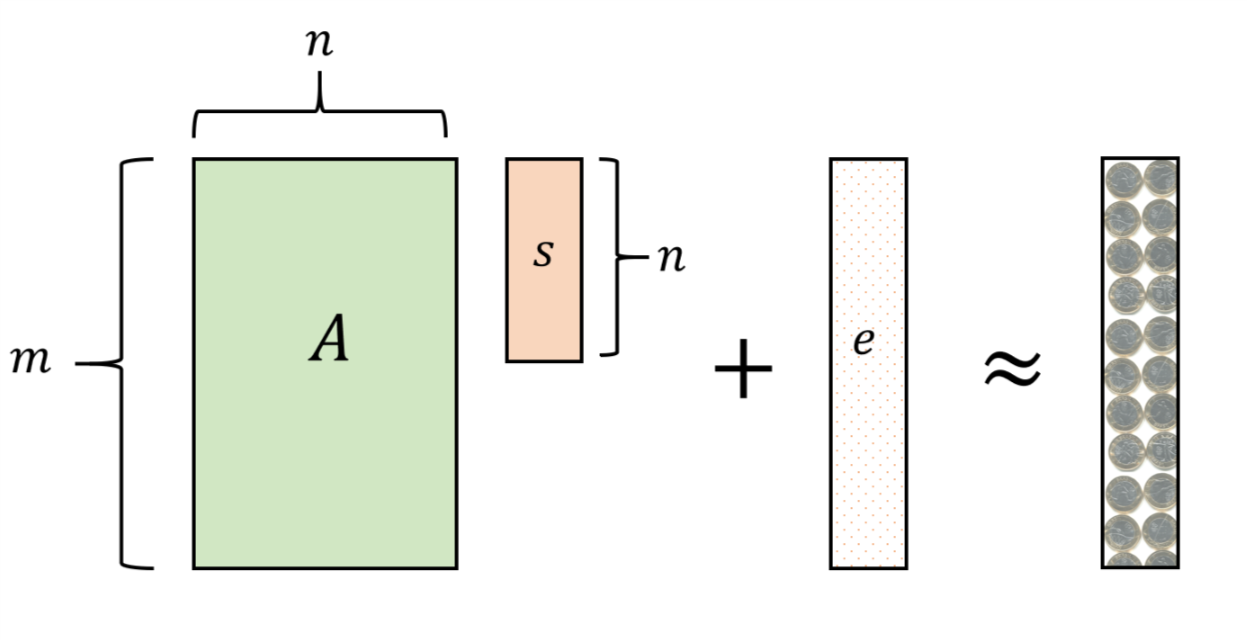
\includegraphics[width=\linewidth, height=1.5in, keepaspectratio]{../figure/lwevecindist.png}
\caption{The search to decision reduction (\cref{LWEsearchtodecthm})
implies that under the LWE conjecture, for every \(m=poly(n)\), if we
choose and fix a random \(m\times n\) matrix \(A\) over \(\Z_q\), the
distribution \(Ax+e\) is indistinguishable from a random vector in
\(\Z_q^m\), where \(x\) is a random vector in \(\Z_q^n\) and \(e\) is a
random ``short'' vector in \(\Z_q^m\). The two distributions are
indistinguishable even to an adversary that knows \(A\).}
\label{figid}
\end{marginfigure}

\hypertarget{LWEsearchtodecthm}{}
\begin{theorem}[Search to decision reduction for LWE] \label[theorem]{LWEsearchtodecthm}

If the LWE conjecture is true then for every \(q=poly(n)\) and
\(\delta=1/poly(n)\) and \(m=poly(n)\), the following two distributions
are computationally indistinguishable:

\begin{itemize}
\item
  \(\{ (A,Ax+e) \}\) where \(A\) is random \(m\times n\) matrix in
  \(\Z_q\), \(x\) is random in \(\Z_q^n\) and \(e\in \Z_q^m\) is random
  noise vector of magnitude \(\delta\).
\item
  \(\{ (A,y) \}\) where \(A\) is random \(m\times n\) matrix in \(\Z_q\)
  and \(y\) is random in \(\Z_q^m\).
\end{itemize}

\end{theorem}

\begin{proof} \label[proof]{Suppose-that-we-had-a-dec}

Suppose that we had a decisional adversary \(D\) that succeeds in
distinguishing the two distributions above with bias \(\epsilon\). For
example, suppose that \(D\) outputs \(1\) with probability
\(p+\epsilon\) on inputs from the first distribution, and outputs \(1\)
with probability \(p\) on inputs from the second distribution.

We will show how we can use this to obtain a polynomial-time algorithm
\(S\) that on input \(m\) noisy equations on \(x\) and a value
\(a\in\ Z_q\), will learn with high probability whether or not the first
coordinate of \(x\) equals \(a\). Clearly, we can repeat this for all
the possible \(q\) values of \(a\) to learn the first coordinate
exactly, and then continue in this way to learn all coordinates.

Our algorithm \(S\) gets as input the pair \((A,y)\) where \(y=Ax+e\)
and we need to decide whether \(x_1 = a\). Now consider the instance
\((A+(r\|0^m\|\cdots \|0^m),y+ar)\), where \(r\) is a random vector in
\(\Z_q^m\) and the matrix \((r\|0^m\|\cdots \|0^m)\) is simply the
matrix with first column equal to \(r\) and all other columns equal to
\(0\). If \(A\) is random then \(A+(r\|0^m\|\cdots \|0^m)\) is random as
well. Now note that \(Ax + (r|0^m\cdots \|0^m)x = Ax + x_1 r\) and hence
if \(x_1 = a\) then we still have an input of the same form
\((A',A'x+e)\).

In contrast, we claim that if if \(x_1 \neq a\) then the distribution
\((A',y')\) where \(A'=A+(r\|0^m\|\cdots \|0^m)\) and
\(y'= Ax + e + ar\) is identical to the uniform distribution over a
random uniformly chosen matrix \(A'\) and a random and independent
uniformly chosen vector \(y'\). Indeed, we can write this distribution
as \((A',y')\) where \(A'\) is chosen uniformly at random, and
\(y'= A'x + e + (a-x_1)r\) where \(r\) is a random and independent
vector. (Can you see why?) Since \(a-x_1 \neq 0\), this amounts to
adding a random and independent vector \(r'\) to \(y'\), which means
that the distribution \((A',y')\) is uniform and independent.

Hence if we send the input \((A',y')\) to our the decision algorithm
\(D\), then we would get \(1\) with probability \(p+\epsilon\) if
\(x_1=a\) and an output of \(1\) with probability \(p\) otherwise.

Now the crucial observation is that if our decision algorithm \(D\)
requires \(m\) equations to succeed with bias \(\epsilon\), we can use
\(100mn/\epsilon^2\) equations (which is still polynomial) to invoke it
\(100n/\epsilon^2\) times. This allows us to distinguish with
probability \(1-2^{-n}\) between the case that \(D\) outputs \(1\) with
probability \(p+\epsilon\) and the case that it outputs \(1\) with
probability \(p\) (this follows from the Chernoff bound; can you see
why?). Hence by using polynomially more samples than the decision
algorithm \(D\), we get a search algorithm \(S\) that can actually
recover \(x\).

\end{proof}

\section{An LWE based encryption
scheme}\label{An-LWE-based-encryption-s}

We can now show the secure variant of our original encryption scheme:

\begin{quote} \label[quote]{LWE-based-encryption-LWEE}

\textbf{LWE-based encryption LWEENC:} * \emph{Parameters:} Let
\(\delta(n)=1/n^4\) and let \(q=poly(n)\) be a prime such that LWE holds
w.r.t. \(q,\delta\). We let \(m = n^2\log q\).

\begin{itemize}
\item
  \emph{Key generation:} Pick \(x\in\Z_q^n\). The private key is \(x\)
  and the public key is \((A,y)\) with \(y=Ax+e\) with \(e\) a
  \(\delta\)-noise vector and \(A\) a random \(m\times n\) matrix.
\item
  \emph{Encrypt:} To encrypt \(b\in\{0,1\}\) given the key \((A,y)\),
  pick \(w\in\{0,1\}^m\) and output
  \(w^\top A, \langle w,y \rangle+b\floor{q/2}\) (all computations are
  done in \(\Z_q\)).
\item
  \emph{Decrypt:} To decrypt \((a,\sigma)\), output \(0\) iff
  \(|\langle a,x \rangle-\sigma|<q/10\).
\end{itemize}

\end{quote}

\begin{pause} \label[pause]{The-scheme-LWEENC-is-also}

The scheme LWEENC is also described in \cref{lweencdescfig} with
slightly different notation. I highly recommend you stop and verify you
understand why the two descriptions are equivalent.

\end{pause}


\begin{marginfigure}
\centering
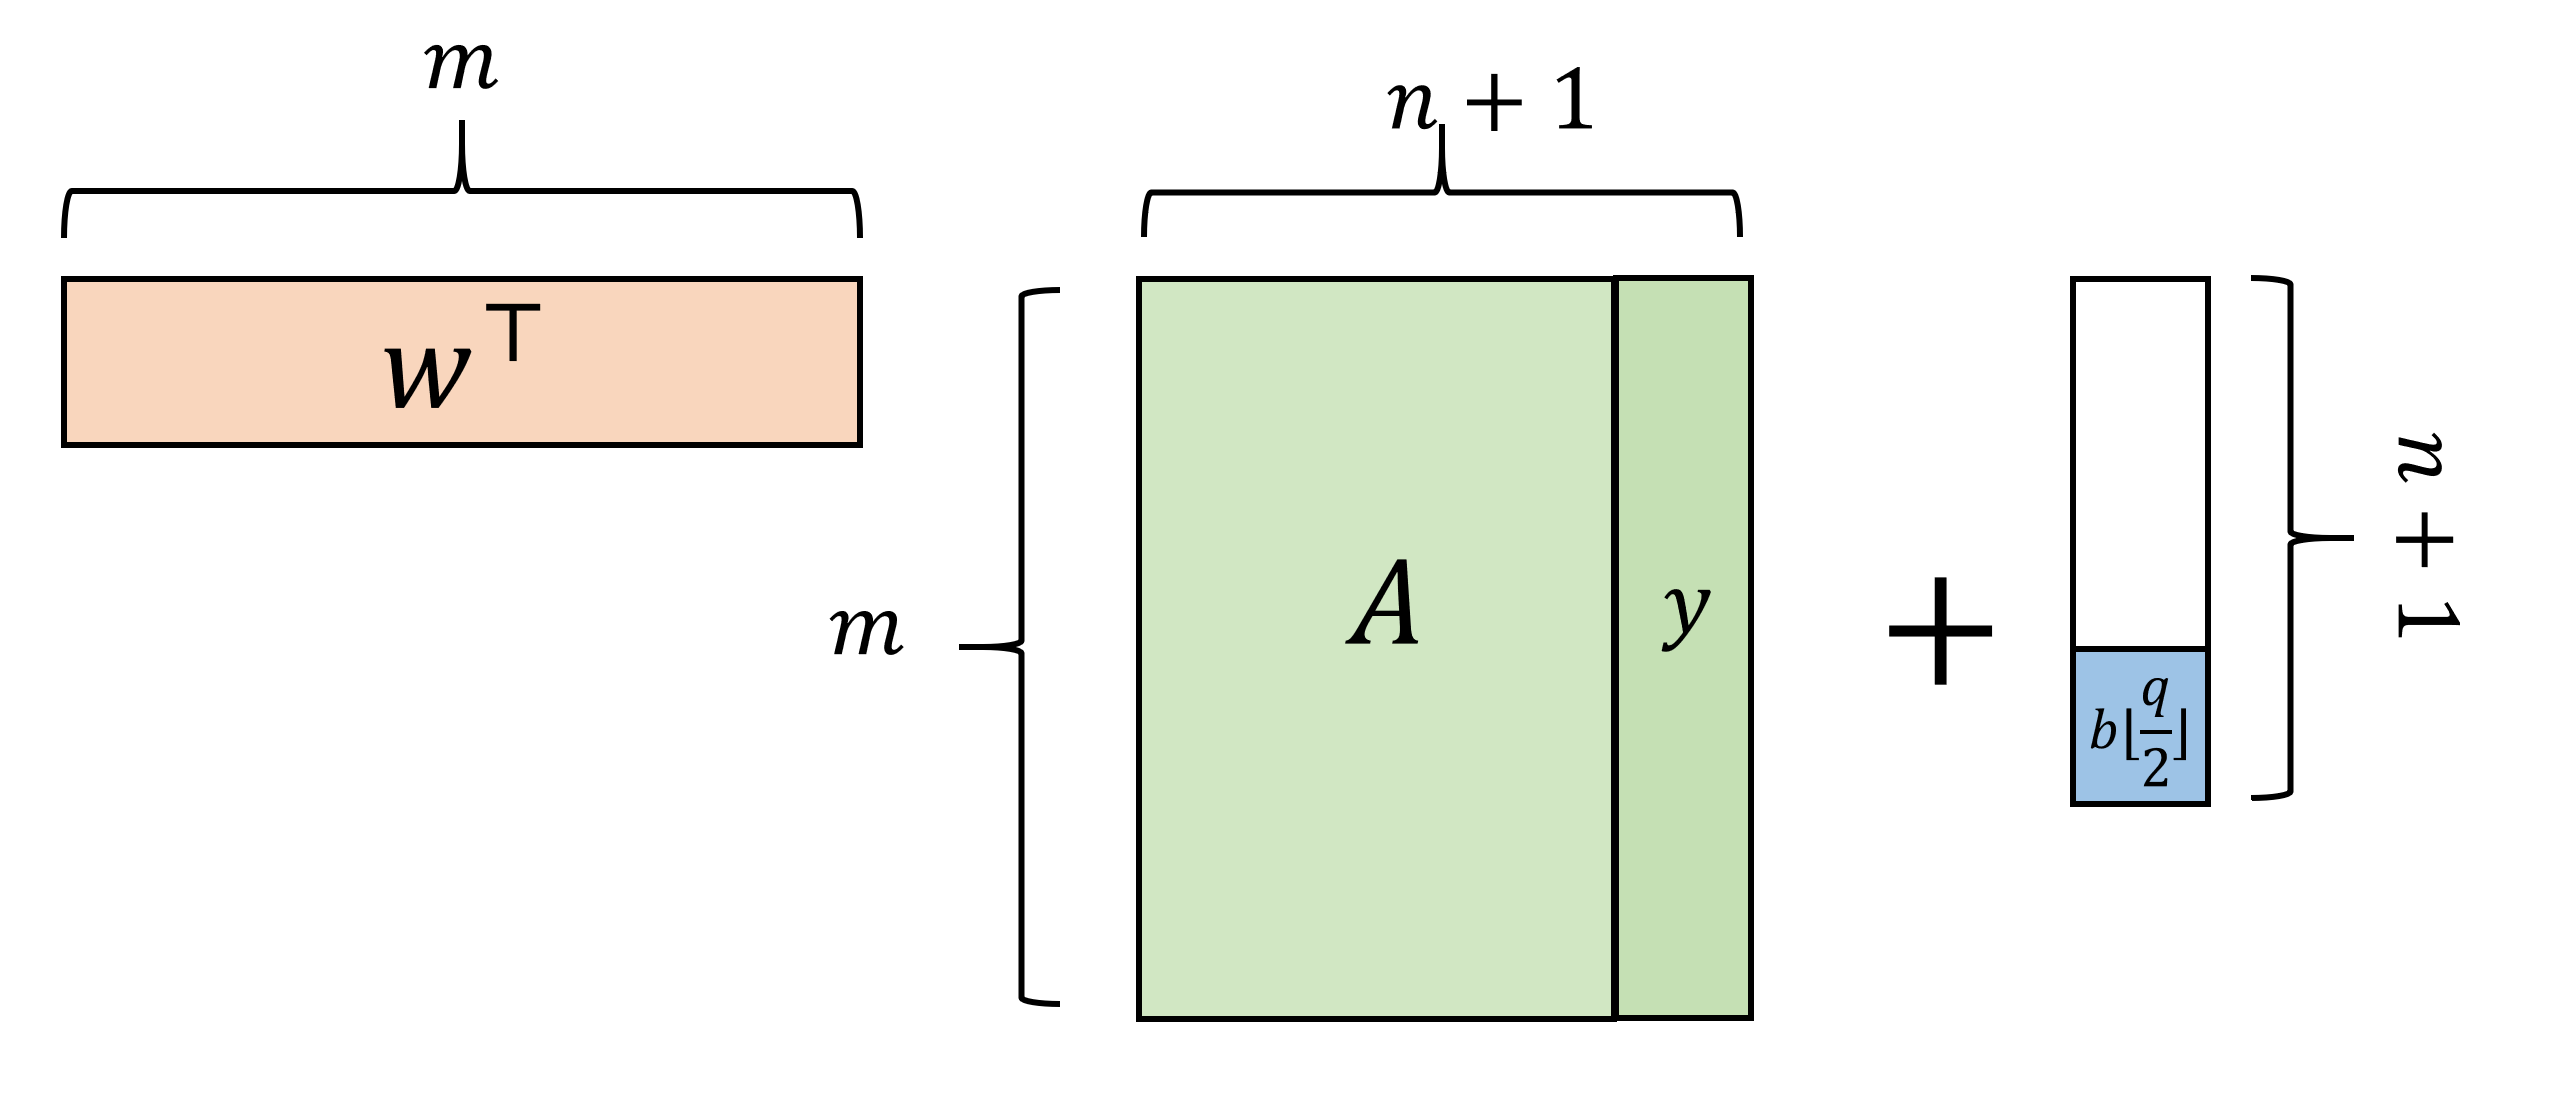
\includegraphics[width=\linewidth, height=1.5in, keepaspectratio]{../figure/lweencdesc.png}
\caption{In the encryption scheme LWEENC, the public key is a matrix
\(A'=(A|y)\), where \(y=As+e\) and \(s\) is the secret key. To encrypt a
bit \(b\) we choose a random \(w \leftarrow_R \{0,1\}^m\), and output
\(w^\top A' + (0,\ldots,0,b\floor{\tfrac{q}{2}})\). We decrypt
\(c \in \Z_q^{n+1}\) to zero with key \(s\) iff
\(|\langle c,(s,-1) \rangle| \leq q/10\) where the inner product is done
modulo \(q\).}
\label{lweencdescfig}
\end{marginfigure}

Unlike our typical schemes, here it is not immediately clear that this
encryption is valid, in the sense that the decrypting an encryption of
\(b\) returns the value \(b\). But this is the case:

\hypertarget{LWEcorrectlem}{}
\begin{lemma} \label[lemma]{LWEcorrectlem}

With high probability, the decryption of the encryption of \(b\) equals
\(b\).

\end{lemma}

\begin{proof} \label[proof]{langle-wtop-Ax-rangle--la}

\(\langle w^\top A,x \rangle = \langle w,Ax \rangle\). Hence, if
\(y=Ax+e\) then
\(\langle w,y \rangle = \langle w^\top A,x \rangle + \langle w,e \rangle\).
But since every coordinate of \(w\) is either \(0\) or \(1\),
\(|\langle w,e \rangle|<\delta m q < q/10\) for our choice of
parameters.\footnote{In fact, due to the fact that the \emph{signs} of
  the error vector's entries are different, we expect the errors to have
  significant cancellations and hence we would expect
  \(|\langle w,e \rangle|\) to only be roughly of magnitude
  \(\sqrt{m}\delta q\), but this is not crucial for our discussions.}
So, we get that if \(a= w^\top A\) and
\(\sigma = \langle w,y \rangle+b\floor{q/2}\) then
\(\sigma - \langle a,x \rangle = \langle w,e \rangle + b\floor{q/2}\)
which will be smaller than \(q/10\) iff \(b=0\).

\end{proof}

We now prove security of the LWE based encryption:

\hypertarget{LWEENCthm}{}
\begin{theorem}[CPA security of LWEENC] \label[theorem]{LWEENCthm}

If the LWE conjecture is true then LWEENC is CPA secure.

\end{theorem}

For a public key encryption scheme with messages that are just bits, CPA
security means that an encryption of \(0\) is indistinguishable from an
encryption of \(1\), even given the public key. Thus \cref{LWEENCthm}
will follow from the following lemma:

\hypertarget{LWEENClem}{}
\begin{lemma} \label[lemma]{LWEENClem}

Let \(q,m,\delta\) be set as in LWEENC. Then, assuming the LWE
conjecture, the following distributions are computationally
indistinguishable:

\begin{itemize}
\item
  \(D\): The distribution over four-tuples of the form
  \((A,y,w^\top A,\langle w,y \rangle)\) where \(A\) is uniform in
  \(\Z_q^{m\times n}\), \(x\) is uniform in \(\Z_q^n\), \(e \in Z_q\) is
  chosen with \(e_i \in \{-\delta q,\ldots,+\delta q\}\), \(y=Ax+e\),
  and \(w\) is uniform in \(\{0,1\}^m\).
\item
  \(\overline{D}\): The distribution over four-tuples
  \((A,y',a,\sigma)\) where all entries are uniform: \(A\) is uniform in
  \(\Z_q^{m\times n}\), \(y'\) is uniform in \(\Z_q^m\), \(a\) is
  uniform in \(\Z_q^n\) and \(\sigma\) is uniform in \(\Z_q\).
\end{itemize}

\end{lemma}

\begin{pause} \label[pause]{You-should-stop-here-and-}

You should stop here and verify that \textbf{(i)} You understand the
statement of \cref{LWEENClem} and \textbf{(ii)} you understand why this
lemma implies \cref{LWEENCthm}. The idea is that \cref{LWEENClem} shows
that the concatenation of the public key and encryption of \(0\) is
indistinguishable from something that is completely random. You can then
use it to show that the concatenation of the public key and encryption
of \(1\) is indistinguishable from the same thing, and then finish using
the hybrid argument.

\end{pause}

We now prove \cref{LWEENClem}, which will complete the proof of
\cref{LWEENCthm}.

\begin{proof}[Proof of \cref{LWEENClem}] \label[proof]{Define-D-to-be-the-distri}

Define \(D\) to be the distribution
\((A,y,w^\top A,\langle w,y \rangle)\) as in the lemma's statement
(i.e., \(y=Ax+e\) for some \(x\), \(e\) chosen as above). Define \(D'\)
to be the distribution \((A,y',w^\top A, \langle w,y' \rangle)\) where
\(y'\) is chosen uniformly in \(\Z_q^m\).

We claim that \(D'\) is computationally indistinguishable from \(D\)
under the LWE conjecture. Indeed by \cref{LWEsearchtodecthm} (search to
decision reduction) this conjecture implies that the distribution \(X\)
over pairs \((A,y)\) with \(y=Ax+e\) is indistinguishable from the
distribution \(X'\) over pairs \((A,y')\) where \(y'\) is uniform. But
if there was some polynomial-time algorithm \(T\) distinguishing \(D\)
from \(D'\) then we can design a randomized polynomial-time algorithm
\(T'\) distinguishing \(X\) from \(X'\) with the same advantage by
setting \(T'(A,y)=T(A,y,w^\top A,\langle w,y \rangle)\) for random
\(w \leftarrow_R \{0,1\}^m\).

We will finish the proof by showing that the distribution \(D'\) is
\emph{statistically indistinguishable} (i.e., has negligible total
variation distance) from \(\overline{D}\). This follows from the
following claim:

\textbf{CLAIM:} Suppose that \(m > 100 n \log q\). If \(A'\) is a random
\(m\times n+1\) matrix in \(\Z_q^m\), then with probability at least
\(1-2^{-n}\) over the choice of \(A'\), the distribution \(Z_{A'}\) over
\(\Z_q^n\) which is obtained by choosing \(w\) at random in
\(\{0,1\}^m\) and outputting \(w^\top A'\) has at most \(2^{-n}\)
statistical distance from the uniform distribution over \(\Z_q^{n+1}\).

Note that the randomness used for the distribution \(Z_{A'}\) is only
obtained by the choice of \(w\), and \emph{not} by the choice of \(A'\)
that is fixed. (This passes a basic ``sanity check'' since \(w\) has
\(m\) random bits, while the uniform distribution over \(\Z_q^n\)
requires \(n \log q \ll m\) random bits, and hence \(Z_{A'}\) at least
has a ``fighting chance'' in being statistically close to it.) Another
way to state the same claim is that the pair \((A',w^\top A')\) is
statistically indistinguishable from the uniform distribution \((A',z)\)
where \(z\) is a vector chosen independently at random from \(\Z_q^n\).

The claim completes the proof of the theorem, since letting \(A'\) be
the matrix \((A|y)\) and \(z=(a,\sigma)\), we see that the distribution
\(D'\), as the form \((A',z)\) where \(A'\) is a uniformly random
\(m\times (n+1)\) matrix and \(z\) is sampled from \(Z_{A'}\) (i.e.,
\(z=w^\top A'\) where \(w\) is uniformly chosen in \(\{0,1\}^m\)). Hence
this means that the statistical distance of \(D'\) from \(\overline{D}\)
(where all elements are uniform) is \(O(2^{-n})\). (Please make sure you
understand this reasoning!)

We will not do the whole proof of the claim (which uses the mod \(q\)
version of the \href{https://goo.gl/KXpccP}{leftover hash lemma} which
we mentioned before and is also ``Wikipedia-able'' - the \textbf{scribe
writers} for this lecture should add those details thogh!) but the idea
is simple. For every \(m\times (n+1)\) matrix \(A'\) over \(\Z_q\),
define \(h_{A'}:\Z_q^m \rightarrow \Z_q^n\) to be the map
\(h_{A'}(w)=w^\top A'\). This collection can be shown to be a ``good''
hash function collection in some specific technical sense, which in
particular implies that for every distribution \(D\) with much more than
\(n\log q\) bits of min-entropy, with all but negligible probability
over the choice of \(A'\), \(h_{A'}(D)\) is statistically
indistinguishable from the uniform distribution. Now when we choose
\(w\) at random in \(\{0,1\}^m\), it is coming from a distribution with
\(m\) bits of entropy. If \(m \gg (n+1)\log q\), then because the output
of this function is so much smaller than \(m\), we expect it to be
completely uniform, and this is what's shown by the leftover hash lemma.

\end{proof}

\begin{pause} \label[pause]{The-proof-of-crefLWEENCth}

The proof of \cref{LWEENCthm} is quite subtle and requires some
re-reading and thought. To read more about this, you can look at the
survey of Oded Regev,
\href{http://www.cims.nyu.edu/~regev/papers/lwesurvey.pdf}{``On the
Learning with Error Problem''} Sections 3 and 4.

\end{pause}

\section{But what are lattices?}\label{But-what-are-lattices}

You can think of a lattice as a discrete version of a subspace. A
lattice \(L\) is simply a discrete subset of \(\mathbb{R}^n\) such that
if \(u,v\in L\) and \(a,b\) are integers then \(au+bv\in L\).\footnote{By
  discrete we mean that points in \(L\) are isolated. One formal way to
  define it is that there is some \(\epsilon>0\) such that every
  distinct \(u,v \in L\) are of distance at least \(\epsilon\) from one
  another.} A lattice is given by a basis which simply a matrix \(B\)
such that every vector \(u\in L\) is obtained as \(u=Bx\) for some
vector of integers \(x\). It can be shown that we can assume without
loss of generality that \(B\) is full dimensional and hence it's an
\(n\) by \(n\) invertible matrix. Note that given a basis \(B\) we can
generate vectors in \(L\), as well as test whether a vector \(v\) is in
\(L\) by testing if \(B^{-1}v\) is an integer vector. There can be many
different bases for the same lattice, and some of them are easier to
work with than others (see \cref{latticebasesfig}).


\begin{marginfigure}
\centering
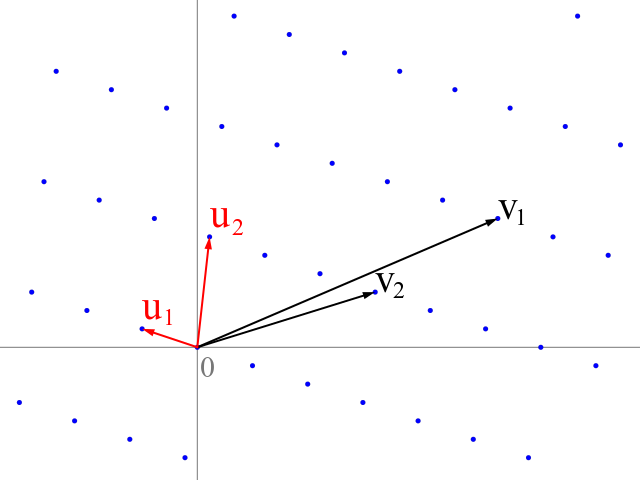
\includegraphics[width=\linewidth, height=1.5in, keepaspectratio]{../figure/Lattice-reduction.png}
\caption{A \emph{lattice} is a discrete subspace \(L \subseteq \R^n\)
that is closed under \emph{integer} combinations. A \emph{basis} for the
lattice is a minimal set \(b_1,\ldots,b_m\) (typically \(m=n\)) such
that every \(u \in L\) is an integer combination of \(b_1,\ldots,b_m\).
The same lattice can have different bases. In this figure the lattice is
a set of points in \(\R^2\), and the black vectors \(v_1,v_2\) and the
ref vectors \(u_1,u_2\) are two alternative bases for it. Generally we
consider the basis \(u_1,u_2\) ``better'' since the vectors are shorter
and it is less ``skewed''.}
\label{latticebasesfig}
\end{marginfigure}

Some classical computational questions on lattices are:

\begin{itemize}
\item
  \emph{Shortest vector problem:} Given a basis \(B\) for \(L\), find
  the nonzero vector \(v\) with smallest norm in \(L\).
\item
  \emph{Closest vector problem:} Given a basis \(B\) for \(L\) and a
  vector \(u\) that is \emph{not} in \(L\), find the closest vector to
  \(u\) in \(L\).
\item
  \emph{Bounded distance decoding:} Given a basis \(B\) for \(L\) and a
  vector \(u\) of the form \(u=v+e\) where \(v\) is in \(L\), and \(e\)
  is a particularly short ``error'' vector (so in particular no other
  vector in the lattice is within distance \(\|e\|\) to \(u\)), recover
  \(v\). Note that this is a special case of the closest vector problem.
\end{itemize}

In particular, if \(V\) is a linear subspace of \(\Z_q^n\), we can think
of it also as a lattice \(\hat{V}\) of \(\mathbb{R}^n\) where we simply
say that that a vector \(\hat{u}\) is in \(\hat{V}\) if all of
\(\hat{u}\)'s coordinates are integers and if we let
\(u_i = \hat{u}_i \pmod{q}\) then \(u\in V\). The learning with error
task of recovering \(x\) from \(Ax+e\) can then be thought of as an
instance of the bounded distance decoding problem for \(\hat{V}\).

A natural algorithm to try to solve the \emph{closest vector} and
\emph{bounded distance decoding} problems is that to take the vector
\(u\), express it in the basis \(B\) by computing \(w = B^{-1}u\), and
then round all the coordinates of \(w\) to obtain an integer vector
\(\tilde{w}\) and let \(v=B\tilde{w}\) be a vector in the lattice. If we
have an extremely good basis \(L\) for the lattice then \(v\) may indeed
be the closest vector in the lattice, but in other more ``skewed'' bases
it can be extremely far from it.

\section{Ring based lattices}\label{Ring-based-lattices}

One of the biggest issues with lattice based cryptosystem is the key
size. In particular, the scheme above uses an \(m\times n\) matrix where
each entry takes \(\log q\) bits to describe. (It also encrypts a single
bit using a whole vector, but more efficient ``multi-bit'' variants are
known.) Schemes using \emph{ideal lattices} are an attempt to get more
practical variants. These have very similar structure except that the
matrix \(A\) chosen is not completely random but rather can be described
by a single vector. One common variant is the following: we fix some
polynomial \(p\) over \(\Z_q\) with degree \(n\) and then treat vectors
in \(\Z_q^n\) as the coefficients of \(n-1\) degree polynomials and
always work modulo this polynomial \(p()\). (By this I mean that for
every polynomial \(t\) of degree at least \(n\) we write \(t\) as
\(ps+r\) where \(p\) is the polynomial above, \(s\) is some polynomial
and \(r\) is the ``remainder'' polynomial of degree \(<n\); then
\(t \pmod{p} = r\).) Now for every fixed polynomial \(t\), the operation
\(A_t\) which is defined as \(s \mapsto ts \pmod{p}\) is a linear
operation mapping polynomials of degree at most \(n-1\) to polynomials
of degree at most \(n-1\), or put another way, it is a linear map over
\(\Z_q^n\). However, the map \(A_d\) can be described using the \(n\)
coefficients of \(t\) as opposed to the \(n^2\) description of a matrix.
It also turns out that by using the Fast Fourier Transform we can
evaluate this operation in roughly \(n\) steps as opposed to \(n^2\).
The ideal lattice based cryptosystem use matrices of this form to save
on key size and computation time. It is still unclear if this structure
can be used for attacks; recent papers attacking principal ideal
lattices have shown that one needs to be careful about this.

One ideal-lattice based system is the
\href{https://newhopecrypto.org/}{``New Hope'' cryptosystem} (see also
\href{https://eprint.iacr.org/2015/1092.pdf}{paper}) that has been
experimented with by Google. People have also made highly optimized
general (non ideal) lattice based constructions, see in particular the
\href{https://frodokem.org/}{``Frodo'' system} (paper
\href{https://eprint.iacr.org/2016/659}{here}, can you guess what's
behind the name?). Both New Hope and Frodo have been submitted to the
\href{https://csrc.nist.gov/Projects/Post-Quantum-Cryptography}{NIST
competition} to select a ``post quantum'' public key encryption
standard.
